\documentclass[11pt]{article}

\usepackage[utf8]{inputenc}
\usepackage[T1]{fontenc}
\usepackage{lmodern}
\usepackage[margin=1in]{geometry}
\usepackage{amsmath,amssymb}
\usepackage{booktabs}
\usepackage{graphicx}
\usepackage{tabularx}
\usepackage{caption}
\usepackage[numbers,sort&compress]{natbib}
\usepackage[hidelinks]{hyperref}
\usepackage{xcolor}

\graphicspath{{figures/}}
\captionsetup{font=small,labelfont=bf}
\newcommand{\bC}{\beta_C}

\title{Do LLM Valuation Agents Read the Filing?\\[2pt]
\large Metamorphic Tests of Filing Fidelity on Korean Listed Firms}
\author{Dong Gyu Park\\
Independent Researcher\\
\texttt{parkdong1015@gmail.com}}
\date{October 2026}

\begin{document}
\maketitle

\begin{abstract}
Large language models (LLMs) are increasingly used to value companies from their filings, but outcome accuracy cannot tell whether a model computes from the filing or recalls what it already knows about the firm. We propose a metamorphic-testing design in which accounting-consistent perturbations of real filings have an exact theoretical effect on per-share value, so the model's response can be measured against a calibrated target. Using 150 Korean listed firms (50 large caps, 50 mid caps and 50 small caps with in-the-money convertible bonds), FY2025 DART filings and a preregistered protocol, we run about 63{,}000 model calls, mostly with Gemini 2.5 Flash-Lite. The primary agent delegates the arithmetic to a Python tool. None of the four preregistered primary hypotheses is supported after Holm correction. Large-cap scale elasticity is 0.993 (95\% CI 0.951--1.035), so values scale with the statements; the firm-memory effect, its dose-response with memory strength, and convertible-bond dilution under-reaction are inconclusive. Exploratory analyses show that the model carries perturbed items into the valuation bridge almost exactly (median 1.00 of the change in cash or non-operating assets), but its projection assumptions vary so much between runs (enterprise value moves by about $\pm4$ times the perturbation) that single-item effects are invisible in a single valuation. Pooled across firms, responses are close to theory for share-count changes (1.007) and non-operating assets (0.875), and larger than theory for cash distributions (1.61). Names pull values toward the price at the training cutoff (stale-anchor coefficient 0.245, $p=0.003$), and agents that compute themselves misreport their own arithmetic in about 98\% of runs. Delegating computation and fixing or averaging assumptions are preconditions for filing-faithful LLM valuation.
\end{abstract}

\noindent\textbf{Keywords:} large language models, equity valuation, metamorphic testing, look-ahead bias, memorization, financial filings, convertible bonds, Korea\\
\textbf{JEL:} G12, G14, C45, M41

\section{Introduction}

LLM agents are being deployed to read company filings and produce valuations, target prices and research reports \citep{zhou2024finrobot,haque2026deep}. Evaluating these agents by comparing their outputs with realized prices or analyst estimates has an identification problem. A model trained on data that include the firm's history can produce an accurate value without using the filing at all \citep{lopezlira2025memorization,gao2025detecting,glasserman2023assessing}. Accuracy therefore confounds two abilities: reading and computing from the disclosed numbers, and recalling what is already known about the company.

We sidestep the problem by asking a different question. Instead of ``is the value right?'' we ask ``does the value change by the right amount when the filing changes?'' This is a metamorphic test \citep{chen2018metamorphic}. We apply perturbations to real filings that preserve accounting identities and have a known theoretical effect on the per-share value of a discounted-cash-flow (DCF) valuation. Examples are scaling every amount by $k$, paying out part of the cash, doubling the share count, adding non-operating assets, and changing the terms of an outstanding convertible bond (CB). The response ratio, the observed change divided by the theoretical change, is a calibrated measure of filing fidelity. It does not require knowing the ``true'' value of the firm.

We combine these tests with information conditions that withhold the firm's name and industry, or replace the name with a fictitious one. These conditions decompose any attenuation of the response into an industry prior, a name effect and a firm-specific memory effect. A memory quiz measures how much the model knows about each firm. Small KOSDAQ firms with convertible bonds provide a setting in which firm-specific memory is weak and the key value driver, dilution, appears only in the filing.

The study is preregistered: hypotheses, sample, prompts, perturbation-size rules and analysis plan were frozen after a pilot (git tag \texttt{prereg-v1}), and every later change is logged. We report all four primary hypotheses, the preregistered exploratory analyses and the robustness checks, and we label the analyses added after seeing the results.

Our results are mostly null for the preregistered hypotheses, and informative about why. With computation delegated to a tool, values scale almost exactly with the statements, and the model transfers each perturbed item into the valuation bridge correctly. However, its projection assumptions vary so much from run to run that the effect of a single disclosed item on the final value is hidden in noise. Averaged across firms, the responses are close to theory, except that cash distributions are over-weighted. We also find that the model's values are pulled toward the firm's price at the training cutoff, and that agents that do their own arithmetic almost never report numbers consistent with their own assumptions.

\paragraph{Contributions.} (i) A calibrated, outcome-free measurement design for filing fidelity of LLM valuation, with accounting-consistent perturbations and theoretical targets. (ii) A decomposition of attenuation into industry, name and firm-memory components, with a memory-strength dose-response test. (iii) Evidence on where the information is lost: the extraction and transfer of perturbed items versus the noise in projection assumptions, and the failure stages of convertible-bond dilution. (iv) A preregistered empirical study on Korean filings (DART), including a memory-poor small-cap setting.

\section{Related Work}

\paragraph{Knowledge conflicts.} NLP work studies how models resolve conflicts between context and parametric memory, typically in single-fact question answering with a binary outcome \citep{longpre2021entity,xie2024adaptive,xu2024survey}. \citet{sun2025task} show that the effect of conflicts depends on the knowledge requirements of the task. Valuation is a multi-step numerical task in which the size of the response, not only its direction, can be measured against a target.

\paragraph{LLMs in investment analysis.} \citet{lee2025yourai} find preferences for technology stocks, large caps and contrarian strategies when models face balanced buy and sell evidence, and attribute part of this to knowledge conflicts. Their outputs are binary decisions on synthetic evidence. \citet{haque2026deep} benchmark deep-research agents against professional reports and find that AI reports fall short. \citet{zhou2024finrobot} build an agent framework for equity research and valuation. We measure the fidelity of the valuation computation itself.

\paragraph{Look-ahead bias and memorization.} \citet{glasserman2023assessing} anonymize headlines and find that company knowledge distracts more than look-ahead bias helps. \citet{lopezlira2025memorization} show that forecasts within the training window cannot separate skill from recall, and \citet{gao2025detecting} propose a statistical test for lookahead propensity. For trading agents, \citet{li2025profit} use counterfactual market perturbations, and \citet{zhu2026knowing} build a memory-controlled benchmark. Our perturbations differ in having exact theoretical response sizes, which yields continuous fidelity measures rather than performance differences.

\section{Measurement Design}

\subsection{Metamorphic relations and metrics}

Let $V$ be the per-share value reported by the agent for a firm under a given input. Each perturbation $\pi$ has a theoretical per-share change $\Delta V^*_\pi$ computed from the agent's own baseline (its median value $V_0$ and share count in the unperturbed cell).

\paragraph{Scale elasticity $\beta$ (E2).} Multiplying every monetary amount of the statements by a factor $k$, with $k \in \{0.5, 0.8, 1, 1.25, 2\}$, leaves margins, growth and leverage unchanged, so a filing-faithful value scales by $k$. For each firm and condition we estimate $\log V_{r} = a + \beta \log k_r + e_r$ by OLS over runs, with HC3 standard errors \citep{mackinnon1985some}. $\beta=1$ is full fidelity; $\beta<1$ is attenuation toward a fixed belief.

\paragraph{Response ratio $R$ (E3).} For single-item perturbations, a cash distribution of $X$ (cash $-X$, equity $-X$, dividend line and DPS updated), an addition of non-operating assets $X$ (FVOCI assets $+X$ against accumulated OCI), and a share split ($m=2$, EPS and DPS divided by 2), we compute
\[ R = \frac{\operatorname{median}(V_{\text{pert}}) - \operatorname{median}(V_{\text{base}})}{\Delta V^*_\pi}, \]
with a percentile bootstrap CI. For cash, $\Delta V^* = -X/N$; for non-operating assets, $+X/N$; for the split, $V_0/m - V_0$.

\paragraph{Self-consistency $\varepsilon$ (E1).} The relative gap between the reported value and the value implied by the agent's own reported cash flows, rates and bridge items.

\paragraph{Decomposition and memory (E4--E6).} Each firm is shown in four conditions: A (name and industry withheld), B (industry label only), D (fictitious name and industry), C (real name and industry). With $\beta$ estimated per condition, total attenuation $\beta_A-\beta_C$ splits into an industry effect $\beta_A-\beta_B$, a name effect $\beta_B-\beta_D$, and a firm-memory effect $E_i=\beta_D-\beta_C$. Memory strength $M_i$ is the mean score of a closed-book quiz (market cap, revenue, operating income, share price, main business, listing market; three repetitions), and identification rates in A, B and D are measured separately (E5).

\paragraph{CB dilution (E8).} For small caps with outstanding CBs, variants V0 (actual CB), V1 (CB removed), V2 (outstanding face increased), V3 (conversion price lowered to a floor-consistent level) and two placebos (a redeemed CB, an irrelevant disclosure) are shown in condition C. The dilution response ratio $R_{dil}$ compares V$j$ with V1 against the if-converted theoretical change, computed from the agent's own equity value and share count; it is defined when the CB is in the money for the agent. A failure-stage classification (E9) labels each run as an extraction, reflection or computation failure, or a success.

\paragraph{Stale anchor (E7).} Regressing $\log V_C$ on $\log V_A$ and the log share price at the model's training cutoff $P_{old}$ tests whether the name pulls the value toward the remembered price.

\subsection{Perturbation size and repetitions}

Perturbations must be large enough to be detected against run-to-run noise $\sigma_i$ and small enough to remain realistic. The preregistered rule sets $X$ to the larger of a precision bound and 5\% of the agent's equity value, capped at 20\% of equity value (and at the firm's cash for distributions). The precision bound is $\sigma_i\sqrt{2/n}/s^*$ times shares, with target standard error $s^*=0.2$. The number of repetitions $n$ is raised from 10 in steps of 5 up to 40 if needed. Firms that cannot meet the bound are excluded from the rule-size cell. Tiered sizes of 2\%, 5\% and 10\% of book equity are run for every firm with positive book equity as a size robustness check.

\section{Data and Experimental Setup}

\paragraph{Sample.} The evaluation date is $T_{post}=$ 2026-04-01; statements are FY2025 (three years shown). The universe is non-financial KOSPI firms and KOSDAQ convertible-bond issuers. We exclude firms halted on $T_{post}$ (KRX daily data), firms failing reported-statement identities, firms with fewer than three years of statements, impaired firms, and firms whose annual report was not filed by $T_{post}$. The sample has 50 large caps (KOSPI market-cap ranks 1--50; median market cap KRW 22.9 trillion), 50 mid caps (KOSPI mid band, stratified by filing-based newsworthiness within cap quintiles; median KRW 0.48 trillion) and 50 small caps (KOSDAQ firms with an in-the-money CB at the KRX close on $T_{post}$, ranked by dilution potential; median KRW 0.09 trillion; dilution median 28.8\%).

\paragraph{Input packages.} Each prompt contains a company block (name and industry, depending on the condition), the balance sheet, income statement and cash-flow statement as reported (KRW million), share information, a notes summary of borrowings and non-operating assets, and, for E8, a CB disclosure generated from structured data (outstanding series, conversion prices, refixing floors). Prices are never shown. Redaction for conditions A, B and D removes every name variant, group name, investee, ticker, homepage and CEO name; an automated check found no identifier in any A/B/D prompt, and identification rates were low (large caps: 3\% in A, 11\% in B, 2\% in D; zero for mid and small caps).

\paragraph{Model and agent structures.} The primary model is \texttt{gemini-2.5-flash-lite} (training cutoff January 2025, temperature 0.3, JSON mode, no thinking), chosen because its cutoff precedes $T_{post}$ by 15 months. Three agent structures are compared: P (plain; the model performs the DCF), R (retrieval; the package is chunked and embedded, and only retrieved chunks are shown) and T (tool; the model returns extracted values, assumptions, yearly FCFF inputs and the dilution decision in one structured call, and Python computes FCFF, end-of-year discounting, a Gordon terminal value, the equity bridge, per-share value and if-converted dilution). The comparison model is \texttt{gemini-3.7-flash}.

\paragraph{Pilot and preregistration.} A pilot on 10 large and 10 small caps (three rounds, about 6{,}000 calls) evaluated five gates. Under structure P, the median self-consistency gap was 81\%, with errors concentrated in discounting, so structure T became the primary structure. Unit slips (amounts reported in billions instead of millions) occurred for the largest firms and were removed by explicit unit rules (prompt v1.1). Most firms report no separate depreciation line, and the model invented depreciation inconsistently, so prompt v1.2 fixes projected depreciation to equal capex. The measurability gate failed (few firms satisfy the size rule), and the preregistered fallback restricts rule-size cells to accepted firms. The hypotheses, sample hash, prompt hashes, size rules and analysis plan were then frozen. Table~\ref{tab:runs} summarizes the runs.

\begin{table}[t]
\centering\small
\caption{Runs. Validity is the share of runs passing schema validation after up to two retries.}
\label{tab:runs}
\begin{tabularx}{\linewidth}{lXrr}
\toprule
Phase & Content & Unique calls & Validity \\
\midrule
Pilot & 3 rounds, 10 L + 10 S firms & $\approx$6{,}000 & 99.8--100\% \\
Main (T, v1.2) & 150 firms: E0/E2 (4 conditions $\times$ 5 $k$ $\times$ 10), E3, E5, E6, E7, E8 & 46{,}670 & 99.4--100\% \\
Extensions & 30 firms (+20 small caps for E8): structures P, R; instruction; E10 & 7{,}480 & 99.7--99.9\% \\
Comparison model & 30 firms, conditions C and D, structure T & 3{,}000 & 100\% \\
\bottomrule
\end{tabularx}
\end{table}

\paragraph{Analysis.} Primary tests (one-sided, $\alpha=0.05$, Holm correction across four hypotheses \citep{holm1979simple}): H1, large-cap $\bC<1$, DerSimonian--Laird random-effects weighted mean \citep{dersimonian1986meta}; H2a, median $E_i>0$ (Wilcoxon signed-rank); H2b, $\gamma_1>0$ in $E_i = \gamma_0 + \gamma_1 M_i + \gamma_2 \ln(\text{cap}_i) + \text{industry FE} + \gamma_3\,\text{id\_rate}^D_i$ (WLS with weights $1/\text{se}(E_i)^2$, HC3); H3, small-cap $R_{dil}<1$ for V0 among firms whose CB is in the money for the agent (DL weighted mean). Firms whose baseline median value is not positive are excluded from log-based measures. A primary hypothesis is ``not supported'' when its 95\% CI excludes effects of practical size (for H1 and H3, a lower bound above 0.9).

\section{Results}

\subsection{Primary hypotheses}

\begin{table}[t]
\centering\small
\caption{Primary hypotheses (structure T, primary model). $p$ values are one-sided.}
\label{tab:primary}
\setlength{\tabcolsep}{4pt}
\begin{tabular}{llrcrrrl}
\toprule
& Statistic & Estimate & 95\% CI & $p$ & $p_{Holm}$ & $n$ & Verdict \\
\midrule
H1 & DL mean $\bC$, large caps ($<1$) & 0.993 & [0.951, 1.035] & 0.376 & 1.000 & 50 & not supported \\
H2a & median $E_i$ ($>0$) & 0.020 & [$-$0.046, 0.095] & 0.428 & 1.000 & 145 & inconclusive \\
H2b & $\gamma_1$ on $M_i$ ($>0$) & 0.096 & [$-$0.550, 0.742] & 0.386 & 1.000 & 145 & inconclusive \\
H3 & DL mean $R_{dil}$, V0 ($<1$) & 0.744 & [$-$0.138, 1.626] & 0.285 & 1.000 & 15 & inconclusive \\
\bottomrule
\end{tabular}
\end{table}

Table~\ref{tab:primary} reports the four primary tests. \textbf{H1 is not supported.} Large-cap values scale with the statements (Figure~\ref{fig:beta}): the weighted mean of $\bC$ is 0.993, the unweighted mean 0.948 and the median 0.981. Under structure T this result has a specific meaning: the model does not change its projection assumptions (growth, margins, discount rate) when the firm becomes larger or smaller, so the delegated arithmetic transmits the scaling.

\begin{figure}[t]
\centering
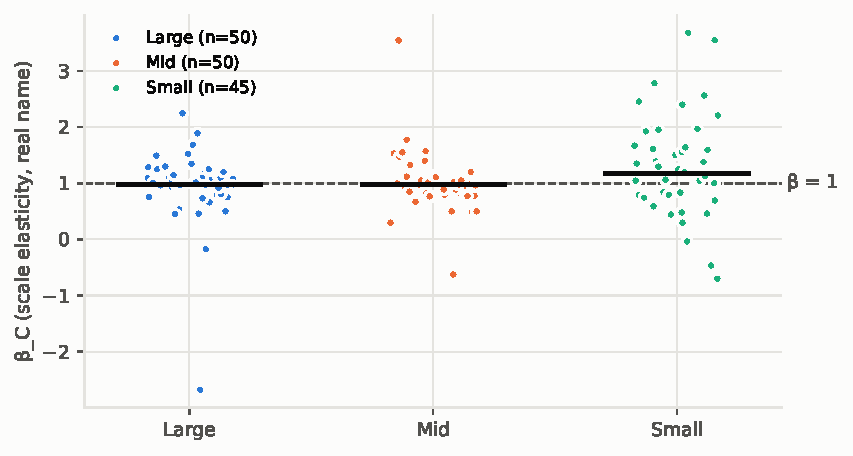
\includegraphics[width=0.72\linewidth]{F2_beta_by_group.pdf}
\caption{Scale elasticity $\bC$ (real name) by size group; bars are medians, the dashed line is $\beta=1$.}
\label{fig:beta}
\end{figure}

\textbf{H2a and H2b are inconclusive.} For large caps, total attenuation $\beta_A-\beta_C$ averages 0.165 and splits evenly into industry (0.050), name (0.053) and firm-memory (0.062) components, but every component's CI includes zero (Figure~\ref{fig:decomp}). Memory strength rises with size ($M_i$: 0.33 large, 0.28 mid, 0.17 small), yet its relation with $E_i$ is weak ($\gamma_1=0.096$, $R^2=0.11$; Figure~\ref{fig:memory}). \textbf{H3 is inconclusive.} Only 15--17 of the 50 small caps have a CB that is in the money at the agent's own value, so power is very low; unweighted estimates are dominated by sign flips around near-zero values.

\begin{figure}[t]
\centering
\begin{minipage}{0.49\linewidth}\centering
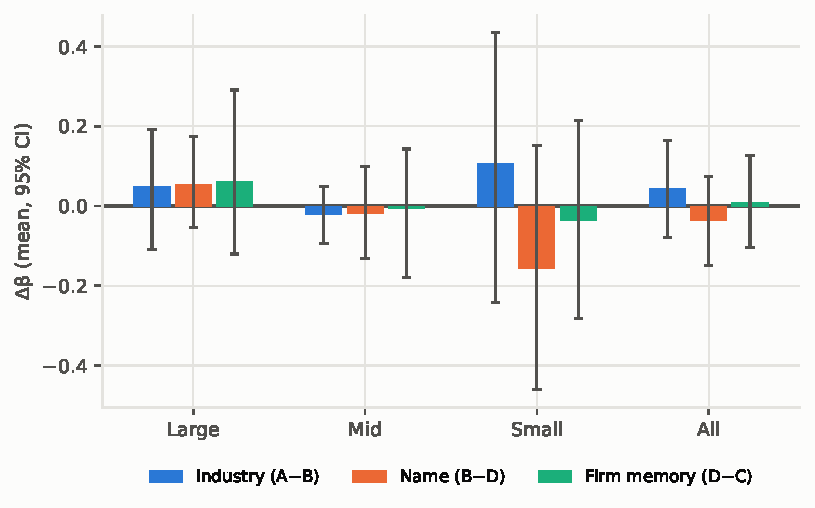
\includegraphics[width=\linewidth]{F3_decomposition.pdf}
\caption{Decomposition of attenuation by group (mean, 95\% bootstrap CI over firms).}
\label{fig:decomp}
\end{minipage}\hfill
\begin{minipage}{0.49\linewidth}\centering
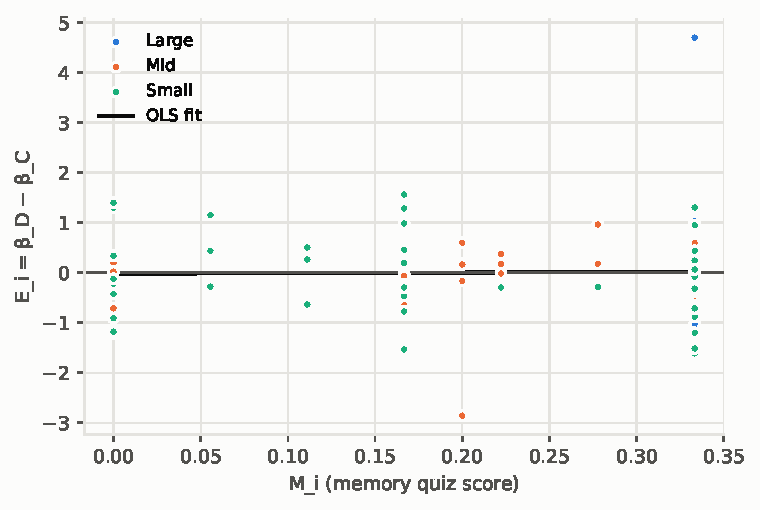
\includegraphics[width=\linewidth]{F4_memory_scatter.pdf}
\caption{Firm-memory effect $E_i$ versus memory strength $M_i$.}
\label{fig:memory}
\end{minipage}
\end{figure}

\subsection{Preregistered exploratory results}

\begin{table}[t]
\centering\small
\caption{Exploratory hypotheses (no multiplicity correction).}
\label{tab:explore}
\begin{tabularx}{\linewidth}{lXl}
\toprule
& Result & Assessment \\
\midrule
H1b & Pooled slope difference small $-$ large $b_S=0.287$ [$-$0.001, 0.574], $p=0.025$ (large-cap slope 1.012) & small caps over-react to scale \\
H1c & $\varepsilon$ large $-$ small (structure P): $-0.148$, $p=0.85$ & not supported \\
H2c & Stale anchor $b_2=0.245$ [0.069, 0.420], $p=0.003$, $n=114$ & supported \\
H2d & Industry effect $\beta_A-\beta_B$: median 0.006, $p=0.25$ & not supported \\
H3b & Failure stages (T, in-the-money small caps): 0\% extraction, reflection or computation failures & no failures \\
H3c & Dose-response slope: mean $-0.26$ [$-$2.16, 1.65] & inconclusive \\
Placebos & 27\% of firm$\times$placebo cells equivalent within $\pm\sigma_i$ & values move with irrelevant text \\
E10 & CB block at the front vs.\ inside a 13{,}000-character filler: difference $-6.5$ KRW, $p=0.90$ & no position effect \\
\bottomrule
\end{tabularx}
\end{table}

Table~\ref{tab:explore} summarizes the exploratory hypotheses. Two results stand out. First, the stale-anchor coefficient is positive and significant: with the real name, values are pulled toward the firm's share price at the training cutoff, controlling for the anonymous value. Second, placebo disclosures (a redeemed CB, an unrelated filing) move values beyond the noise band in most cells, which shows that irrelevant text also perturbs the assumptions.

\paragraph{Agent structures (H4).} On the same 30 firms, structures P and R deviate more from $\beta=1$ than T (median paired $|1-\bC|$ differences 0.060 and 0.030, $p=0.17$ and $0.13$). The clearest difference lies in arithmetic. P and R report values inconsistent with their own assumptions, with median $\varepsilon$ of 0.76 and 0.77, and the failure-stage classification attributes 98.5\% (P) and 97.8\% (R) of runs to computation failures, against 0\% for T (Figure~\ref{fig:stages}).

\begin{figure}[t]
\centering
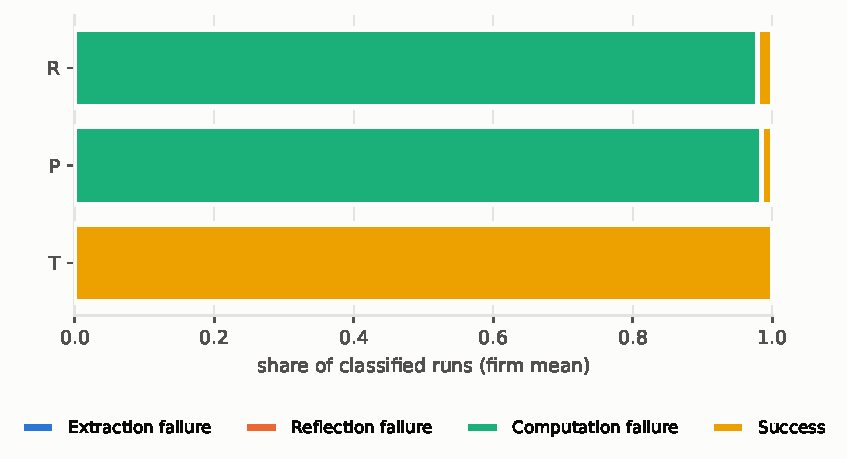
\includegraphics[width=0.66\linewidth]{F6_stages.pdf}
\caption{E9 failure stages by agent structure (CB variants, small caps; firm means).}
\label{fig:stages}
\end{figure}

\subsection{Response fidelity to single disclosed items (added after the results)}

The central question of the study is whether values change by the right amount when a disclosed item changes. Firm-level response ratios are too imprecise to answer it firm by firm. Run-to-run variation of the baseline value has a median coefficient of variation of 26\% for large caps, 36\% for mid caps and 103\% for small caps, against perturbations of 2--20\% of equity. In addition, only 8 (cash) and 28 (non-operating) firms met the size rule. During this analysis we also found that the tier runs, preregistered for every firm, had been attached only to rule-size firms; the missing 6{,}790 calls were run before the analyses below. We report two analyses that were \emph{not} preregistered.

\paragraph{Pooled response ratios.} Each firm-cell $R$ has a bootstrap CI; we take its width divided by 3.92 as the standard error, combine a firm's cells by inverse variance, and pool firms with the DL random-effects mean (Table~\ref{tab:pooled}, Figure~\ref{fig:pooled}). Share-count changes are reflected exactly ($R=1.007$, homogeneous across firms). Non-operating assets are reflected on average ($0.875$; large caps $0.64$, below 1 at $p=0.04$). Cash distributions are over-weighted on average ($1.61$, above 1 at $p=0.012$, with high heterogeneity, $I^2=0.81$). Rule-size cash cells, the most precise, give 1.07 [0.84, 1.30]. CB dilution remains undetermined.

\begin{table}[t]
\centering\small
\caption{Pooled response ratios across firms (DL random effects; exploratory). Tests are two-sided.}
\label{tab:pooled}
\begin{tabular}{lrcrrrr}
\toprule
Perturbation & $\bar R$ & 95\% CI & $p$ vs.\ 1 & $p$ vs.\ 0 & Firms & $I^2$ \\
\midrule
Share split ($m=2$) & 1.007 & [0.995, 1.018] & 0.26 & $<$0.001 & 122 & 0.00 \\
Non-operating assets & 0.875 & [0.609, 1.141] & 0.36 & $<$0.001 & 122 & 0.86 \\
\quad large caps & 0.637 & [0.286, 0.988] & 0.04 & $<$0.001 & 46 & 0.87 \\
Cash distribution & 1.612 & [1.134, 2.089] & 0.012 & $<$0.001 & 119 & 0.81 \\
\quad rule-size cells & 1.068 & [0.837, 1.298] & 0.57 & $<$0.001 & 8 & 0.37 \\
CB dilution V0 & 0.744 & [$-$0.138, 1.626] & 0.57 & 0.10 & 15 & 0.60 \\
CB dilution V2 (face up) & 0.361 & [$-$0.332, 1.054] & 0.07 & 0.31 & 15 & 0.76 \\
CB dilution V3 (price down) & 1.145 & [0.311, 1.979] & 0.73 & 0.007 & 16 & 0.72 \\
\bottomrule
\end{tabular}
\end{table}

\begin{figure}[t]
\centering
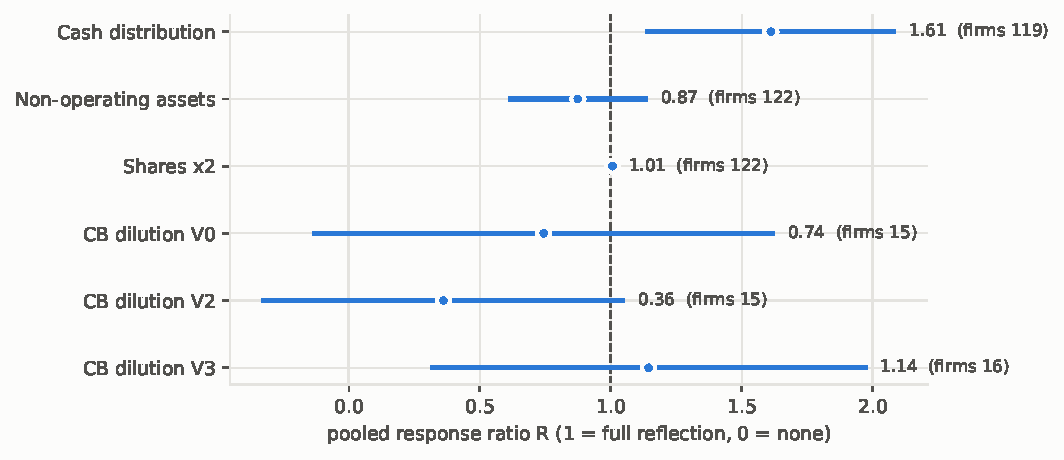
\includegraphics[width=0.74\linewidth]{F8_pooled.pdf}
\caption{Pooled response ratios (DL random effects, 95\% CI); 1 is full reflection.}
\label{fig:pooled}
\end{figure}

\paragraph{Channel decomposition.} Under structure T, equity value equals enterprise value (EV) minus net debt plus non-operating assets. Net debt and non-operating assets are read from the filing, and EV follows from the model's projection assumptions. Dividing the change between perturbed and baseline cells by $X$:
\begin{itemize}
\item \textbf{Cash distributions.} The change in net debt has median 1.00 (IQR 1.00--1.00; 390 cells).
\item \textbf{Non-operating assets.} The change in the non-operating assets added in the bridge has median 1.00 (at least 0.9 in 95.8\% of 478 cells).
\item \textbf{Enterprise value.} EV changes with a median near zero (0.14 and $-0.00$) but an IQR of about $\pm4X$ for both perturbations.
\end{itemize}
The disclosed change therefore reaches the right place in the computation. The imprecision of $R$ comes from assumption noise in EV, not from a failure to read or apply the filing.

\section{Robustness}

All primary conclusions survive the preregistered robustness checks:
\begin{itemize}
\item \textbf{R1, identified firms.} Excluding firms with identification rate $\geq 0.5$ (1--2 firms) leaves H2a and H2b unchanged.
\item \textbf{R2, perturbation size.} Tier size and $R$ are uncorrelated (Spearman $0.04$, $p=0.22$, 832 cells).
\item \textbf{R3, half the repetitions.} Large-cap mean $\bC$ falls to $0.855$ [0.597, 1.043], showing the instability of fewer repetitions.
\item \textbf{R4, anomaly-flagged runs.} Excluding them (45\% of runs) gives H1 $0.996$ and H2a $0.029$.
\item \textbf{R5, comparison model.} On 30 firms the comparison model gives median $\bC$ $0.979$ ($p=0.03$ for $<1$) and median $E_i$ $0.033$ ($p=0.14$).
\item \textbf{R6, instruction.} An instruction to use only the provided data lowers $\bC$ under structure P by $0.28$ ($p=0.036$).
\item \textbf{R8, low-validity cells.} Excluding them changes nothing.
\item \textbf{R9, median-based $\beta$.} The large-cap mean is $1.009$.
\end{itemize}
The robustness check that excludes complex CBs (R7) could not be run because call and net-settlement features are not available in structured form. For the memory quiz, H2b's $\gamma_1$ is 0.23 without the main-business item, 0.44 with automatically drafted keywords and 0.10 with researcher-reviewed keywords; all CIs include zero.

\section{Discussion}

\paragraph{What the agent gets right.} With arithmetic delegated, the model extracts the disclosed numbers, keeps its assumptions stable under proportional scaling, and transfers single-item changes into the valuation bridge almost exactly. This is a meaningful form of filing fidelity: the information in the filing reaches the computation.

\paragraph{What hides it.} The projection assumptions are re-drawn in every run, and irrelevant text moves them too, as the placebo results show. The resulting noise in enterprise value is several times larger than the effect of a typical disclosed item, so a single valuation cannot be said to reflect a 5\% change in the balance sheet, even though the computation does. For practitioners, this argues for three practices: (i) delegating arithmetic to tools; (ii) fixing or externally setting the assumptions, or reporting medians over many runs; (iii) auditing intermediate quantities (net debt, non-operating assets, diluted shares) rather than the final value.

\paragraph{Memory.} The decomposition and dose-response tests do not establish a firm-memory effect on how values respond to the filing. However, the stale-anchor result shows that the name moves the level of the value toward remembered prices. Memory thus appears to affect where the value sits more than how it responds.

\paragraph{Limitations.}
\begin{itemize}
\item \textbf{Scope.} One primary model, which is closed-weight (a deviation from our plan for an open-weight model), one valuation method (five-year FCFF DCF), and one evaluation date.
\item \textbf{Depreciation.} Projected depreciation equal to capex is a researcher-imposed assumption, and the model complied in 68\% of pilot runs.
\item \textbf{Anomaly flags.} The model flagged ``data anomalies'' in 54--87\% of runs, including unperturbed inputs, so the flags carry no information about manipulation detection.
\item \textbf{Comparison model.} Its training cutoff (March 2026) is close to $T_{post}$, so it is a robustness check, not a time-based identification.
\item \textbf{Convertible bonds.} The CB analyses are under-powered because few CBs are in the money at the agent's own values.
\item \textbf{Exclusions.} An administrative-issue exclusion rule was not applied.
\item \textbf{Memory quiz.} The main-business item was scored against keywords drafted from annual reports by an LLM and reviewed by the author, who often added the model's own phrasing; its correct rates (96\%, 84\% and 32\% for large, mid and small caps) should be read as upper bounds.
\item \textbf{Post-hoc analyses.} The pooled and channel analyses were not preregistered.
\end{itemize}

\section{Conclusion}

Metamorphic tests with calibrated targets make it possible to measure whether an LLM valuation agent uses the filing, without relying on outcome accuracy. In a preregistered study of 150 Korean firms, a tool-assisted agent read and transferred disclosed changes correctly and scaled values with the statements. Its run-to-run assumption noise, however, hid single-item effects in any single valuation, and the firm's name pulled values toward the price at the training cutoff. Filing-faithful LLM valuation requires delegated computation and controlled assumptions, and it should be evaluated on intermediate quantities as well as on final values.

\section*{Data, code and preregistration}
The preregistration (\texttt{docs/preregistration.md}, git tag \texttt{prereg-v1}), decisions log, prompts with SHA-256 hashes, analysis code and derived firm-level data accompany this paper (repository: \url{https://github.com/caxios/llm-FSA-evaluation}). Raw DART and KRX data are not redistributed and can be re-fetched with the provided scripts.

\section*{Use of AI tools}
LLMs are the object of study. In addition, the author used an AI coding assistant for software development, data processing and drafting. The author designed the study, reviewed all code, results and text, and takes full responsibility for the content.

\bibliographystyle{plainnat}
\bibliography{references}

\end{document}
